\documentclass{standalone}
\usepackage{xstring}
\usepackage{tikz}
\usetikzlibrary{shapes}
\usetikzlibrary{arrows.meta}

\newcommand{\singletons}[2]{
	\begin{tikzpicture}
		\foreach \i in {18, 90, 162, 234, 306} {
			\node[draw, circle, inner sep = 1.25pt]  (\i) at (\i:0.2) {};
		}
		\IfEqCase{#1}{
			{A}{\node[draw, circle, inner sep = 1.25pt, fill=black]  (A) at (90:0.2) {};}
			{B}{\node[draw, circle, inner sep = 1.25pt, fill=black]  (B) at (18:0.2) {};}
			{C}{\node[draw, circle, inner sep = 1.25pt, fill=black]  (C) at (306:0.2) {};}
			{D}{\node[draw, circle, inner sep = 1.25pt, fill=black]  (D) at (234:0.2) {};}
			{E}{\node[draw, circle, inner sep = 1.25pt, fill=black]  (E) at (162:0.2) {};}
			
		};
		\IfEqCase{#2}{
			{A}{\node[draw, circle, inner sep = 1.25pt, fill=black]  (A) at (90:0.2) {};}
			{B}{\node[draw, circle, inner sep = 1.25pt, fill=black]  (B) at (18:0.2) {};}
			{C}{\node[draw, circle, inner sep = 1.25pt, fill=black]  (C) at (306:0.2) {};}
			{D}{\node[draw, circle, inner sep = 1.25pt, fill=black]  (D) at (234:0.2) {};}
			{E}{\node[draw, circle, inner sep = 1.25pt, fill=black]  (E) at (162:0.2) {};}	
		};
	\end{tikzpicture}
}

\begin{document}

	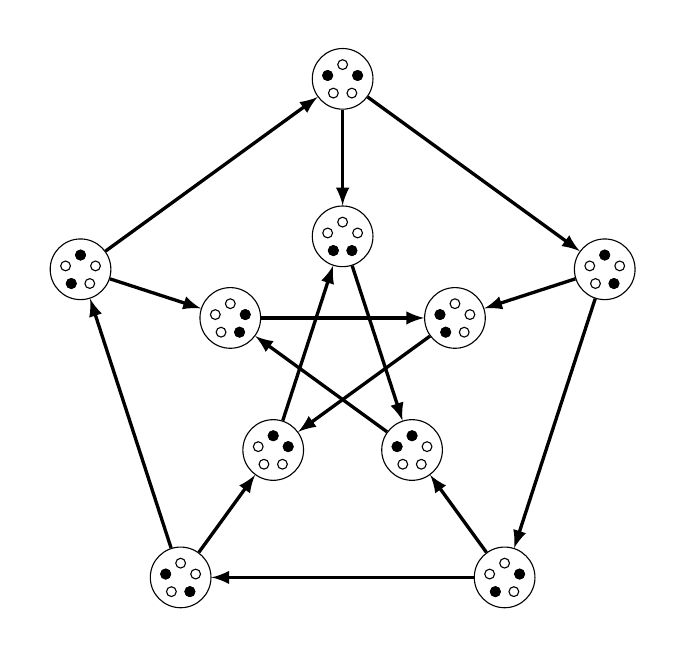
\begin{tikzpicture}
		\path (-4.0, -3.5) -- (-4.0, 4.15) -- (4.0, 4.15) -- (4.0, -3.5) -- cycle;
		\node[draw, circle, inner sep = 0.5pt]  (CD) at (90:1.5) {\singletons{C}{D}};
		\node[draw, circle, inner sep = 0.5pt]  (BC) at (162:1.5) {\singletons{B}{C}};
		\node[draw, circle, inner sep = 0.5pt]  (AB) at (234:1.5) {\singletons{A}{B}};
		\node[draw, circle, inner sep = 0.5pt]  (EA) at (306:1.5) {\singletons{E}{A}};
		\node[draw, circle, inner sep = 0.5pt]  (DE) at (18:1.5) {\singletons{D}{E}};
		\draw[very thick,  -latex] (AB) to (CD);
		\draw[very thick,  -latex] (CD) to (EA);
		\draw[very thick,  -latex] (EA) to (BC);
		\draw[very thick,  -latex] (BC) to (DE);
		\draw[very thick,  -latex] (DE) to (AB);

		\node[draw, circle, inner sep = 0.5pt]  (EB) at (90:3.5) {\singletons{E}{B}};
		\node[draw, circle, inner sep = 0.5pt]  (DA) at (162:3.5) {\singletons{D}{A}};
		\node[draw, circle, inner sep = 0.5pt]  (CE) at (234:3.5) {\singletons{C}{E}};
		\node[draw, circle, inner sep = 0.5pt]  (BD) at (306:3.5) {\singletons{B}{D}};
		\node[draw, circle, inner sep = 0.5pt]  (AC) at (18:3.5) {\singletons{A}{C}};
		\draw[very thick,  -latex] (AC) to (BD);
		\draw[very thick,  -latex] (BD) to (CE);
		\draw[very thick,  -latex] (CE) to (DA);
		\draw[very thick,  -latex] (DA) to (EB);
		\draw[very thick,  -latex] (EB) to (AC);
%		
		\draw[very thick,  -latex] (EB) to (CD);
		\draw[very thick,  -latex] (DA) to (BC);
		\draw[very thick,  -latex] (CE) to (AB);
		\draw[very thick,  -latex] (BD) to (EA);
		\draw[very thick,  -latex] (AC) to (DE);
	\end{tikzpicture}

\end{document}